\section{Genetic Algorithm}

A genetic algorithm (GA) is a search heuristic that is based on Darwin's theory of natural evolution. Darwin theorized that over a period of time a population of individuals would naturally mate and create offspring that were better than themselves. He suggests that not all individuals are created equally and that eventually the weaker individuals would die off. This same principle can be applied to a search algorithm. A GA contains a population of individuals that are evolved to find improved candidate solutions.

The individuals of a GA represent possible candidate solutions to the problem. Individuals are refered to as chromosomes. Typically a chromosome is represented as an array where each index of the array represents a property of the candidate solution. There are no restrictions to the encoding of a chromosome but each property of the chromosome must be independant from the others. The simplest example of a representation is a binary array of 1's and 0's, as shown in Figure~\ref{fig:sampleChromosome}.

\begin{figure}[H]
  \label{fig:sampleChromosome}
  \centering
  \begin{tabular}{ | l | l | l | l | l | l | l | l | }
    \hline
    0 & 1 & 1 & 0 & 1 & 0 & 1 & 0 \\
    \hline
  \end{tabular}
  \caption{Simple Chromosome Represention}
\end{figure}

Finding a representation is only the first step in creating a genetic algorithm. The next step is to define your set of operators. A GA consists of multiple operators that assist in the evolution of the population. Figure~\ref{fig:gaFlowchart} depicts the flowchart of a genetic algorithm and where each genetic operation is performed.

\begin{figure}[H]
	\centering
	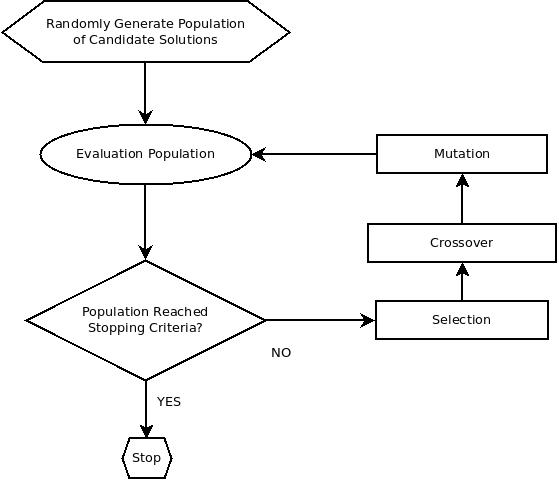
\includegraphics[bb=0 0 310 207,scale=0.5]{figures/GA.jpeg}
	\caption{Population Individual Modification}
	\label{fig:gaFlowchart}
\end{figure}

\subsection{Genetic Operators}

Each of the following operators represent a piece of a genetic algorithm. They facilitate the evolutionary process in an effort to find better candidate solutions. Each of these operators has a unique purpose in the search algorthm but there are many different types of ways these goals can be carried out. Only a few of the different methods will be described in this work.

\textit{Selection Operator}: This operator is very important to the \textit{Crossover} and \textit{Mutation} operators. The idea behind this operator is to put selectionary pressure on the population during the evolutionary process. Individuals with a better fitness score should be allowed a better chance of breeding to create the next population. During the selection process two individuals are chosen breeding or reproduction. There are several selection methods but in this only \textit{k-Tournament selection} will be explained.

The \textit{k}-Tournament selection method works by randomly selecting \textit{k} individuals from the population, where \textit{k} is less than the number of individuals in the population, and selecting the individual that has the best fitness score from the \textit{k} individuals. The value of \textit{k} should be relatively small compared to the size of the population. If the value of \textit{k} is too large it would defeat the purpose of this selection method. For example, if there is a population size of 100 the value of \textit{k} should be around 2-5.

\textit{Crossover Operator}: This operator is essential to evolving the individuals of the population. Crossover is how two individuals breed to create two new individuals. With respect to the evolutionary process, crossover exploits the current information that is contained within the population in order to find improved individuals. The most widely used type of crossover is N-point crossover.

N-point crossover works by randomly selecting N cutting points and swapping the information between the two individuals along those N points. Figure~\ref{fig:2PointCrossover} demonstrates how the swapping of information occurs during 2-point crossover.

\begin{figure}[H]
  \centering
  \begin{tabu}{ | l | l | l |[2pt] l | l | l |[2pt] l | l | l | }
    \hline
    Parent 1 & \textcolor{blue}{0} & \textcolor{blue}{1} & \textcolor{blue}{1} & \textcolor{blue}{0} & \textcolor{blue}{1} & \textcolor{blue}{0} & \textcolor{blue}{1} & \textcolor{blue}{0} \\ \hline
    Parent 2 & \textcolor{red}{0} & \textcolor{red}{0} & \textcolor{red}{1} & \textcolor{red}{0} & \textcolor{red}{0} & \textcolor{red}{1} & \textcolor{red}{0} & \textcolor{red}{0} \\ \hline
  \end{tabu}
  \\
  \vspace{3 mm}
  \line(1,0){250}
  \\
  \vspace{3 mm}
  \begin{tabu}{ | l | l | l |[2pt] l | l | l |[2pt] l | l | l | }
    \hline
    Child 1 & \textcolor{red}{0} & \textcolor{red}{0} & \textcolor{blue}{1} & \textcolor{blue}{0} & \textcolor{blue}{1} & \textcolor{red}{1} & \textcolor{red}{0} & \textcolor{red}{0} \\ \hline
    Child 2 & \textcolor{blue}{0} & \textcolor{blue}{1} & \textcolor{red}{1} & \textcolor{red}{0} & \textcolor{red}{0} & \textcolor{blue}{0} & \textcolor{blue}{1} & \textcolor{blue}{0} \\ \hline
  \end{tabu}
  \caption{2-Point Crossover}
  \label{fig:2PointCrossover}
\end{figure}

\textit{Mutation Operator}: The mutation operator is used to introduce random changes to the individuals during evolution. Mutations to individuals are a way to explore the search space. Depending on how the initial population was created there may not be the necessary information in the population to find the optimal solution with crossover alone. Mutations allow for new information to possibly be introduced into the population. A common type of mutation is single-point mutation where a single index in your individual is modified. Figure~\ref{fig:mutation} demonstrates single-point mutation.

\begin{figure}[H]
  \centering
  \begin{tabular}{ | l | l | l | l | l | l | l | l | l | }
    \hline
    Individual & 0 & 1 & 1 & 0 & 1 & 0 & 1 & 0 \\
    \hline
  \end{tabular}
  \\
  \vspace{3 mm}
  \line(1,0){250}
  \\
  \vspace{3 mm}
  \begin{tabular}{ | l | l | l | l | l | l | l | l | l | }
    \hline
    Mutant & 0 & 1 & 1 & \textcolor{red}{1} & 1 & 0 & 1 & 0 \\
    \hline
  \end{tabular}
  \caption{Single-point Mutation}
  \label{fig:mutation}
\end{figure}

\textit{Elitism Operator}: During each generation of the genetic algorithm a new population is created using the individuals from the population in the previous generation. The new population is bred from the previous individuals with the hopes of creating better individuals. Sometimes this is not the case and the population can end up losing valuable information from individuals that were not chosen during the selection process. To prevent this from happening the elitism operator was create. The elitism operator works by seeding the next generations population with the individuals with the best fitness score. Typically only the top 1\% of individuals are copied into the next generation.